\documentclass{article}

% \usepackage[margin=0.75in]{geometry}
\usepackage{xcolor}
\usepackage{graphicx}
\usepackage{textgreek}

\renewcommand{\labelitemi}{-}

\title{\textbf{Biologie}}

\graphicspath{ {./images/} }

\begin{document}
\maketitle
    \section{Enzymatik}
    \textbf{Enzyme} sind Moleküle die Stoffwechselprozesse im Körper beschleunigen.
    Dies bewirken sie indem sie die \textbf{Aktivierungsenergie} einer Reaktion herabsetzen.
    Die meisten Enzyme sind \textbf{Proteine}.
    Wie alle Proteine bestehen auch Enzyme aus 21 verschidenen Aminosäuren, die sich zu langen \textbf{Aminosäuresequenzen} verbinden können. 
    Da Enzyme unverändert aus der Reaktion, die sie beschleunigen, hervorgehen, nennt man sie auch \textbf{Biokatalysatoren}.
    Bei einer enzymatisch gesteuerten Reaktion lagert sich das Substrat im \textbf{aktiven Zentrum} eines Enzyms an und die umbildung des Substrats findet statt.
    \filbreak
    \subsection{Bennenung}
    Die Enzyme werder häufig nach folgendem Muster benannt: \[\textcolor{red}{Substrat} + \textcolor{blue}{Wirkung} + \textcolor{green}{ase} \]
    \begin{center}
        Bsp.:\textcolor{red}{Aminosäure}-\textcolor{blue}{Oxid}\textcolor{green}{ase}
    \end{center}
    \filbreak
    \subsection{Wirkungs- und Substratspezifität}
    Enzyme arbeiten \textbf{wirkungsspezifisch}, das heißt sie katalysieren immer genau eine Reaktionstyp.
    Außerdem arbeiten sie \textbf{substratspezifisch}, das bedeutet sie katalysieren immer Reaktionen mit einem spezifischen Substrat.
    \filbreak
    \subsection{Struktur}
    Hierbei bertrachtet man (im Lehrplan) 3 "Ebenen":\\
    \begin{itemize}
        \item Primärstruktur: Aminosäure-Sequenz \\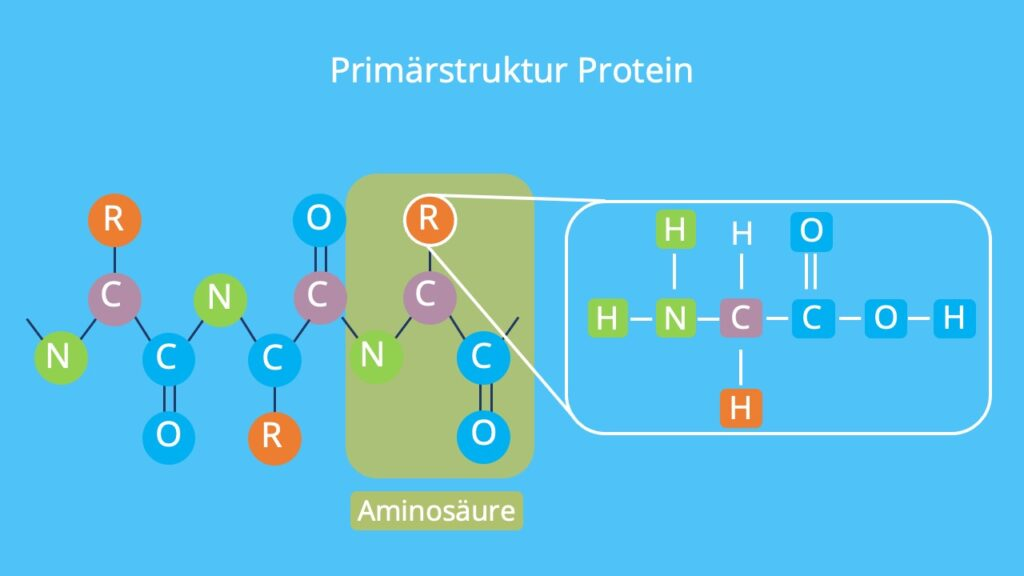
\includegraphics[scale=0.25]{Proteine_Primär}
        \item Sekundärstruktur: \textalpha-Helix- und \textbeta-Faltblatt-Struktur \\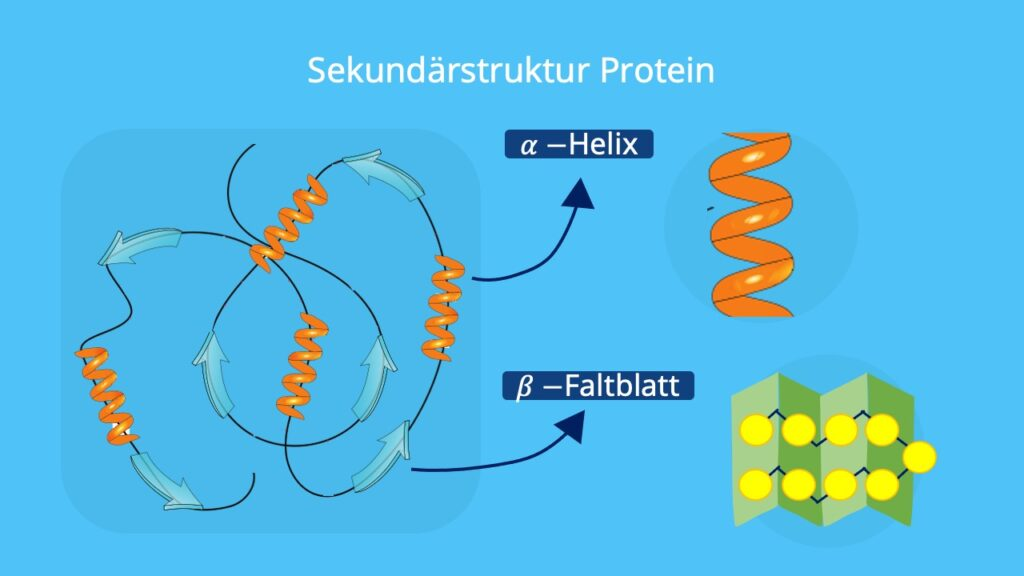
\includegraphics[scale=0.25]{Proteine_Sekundär}
        \item Tertiärstruktur: räumliche Struktur des Proteins durch Ausbildung von intramolekularen Bindungen und Wechselwirkungen \\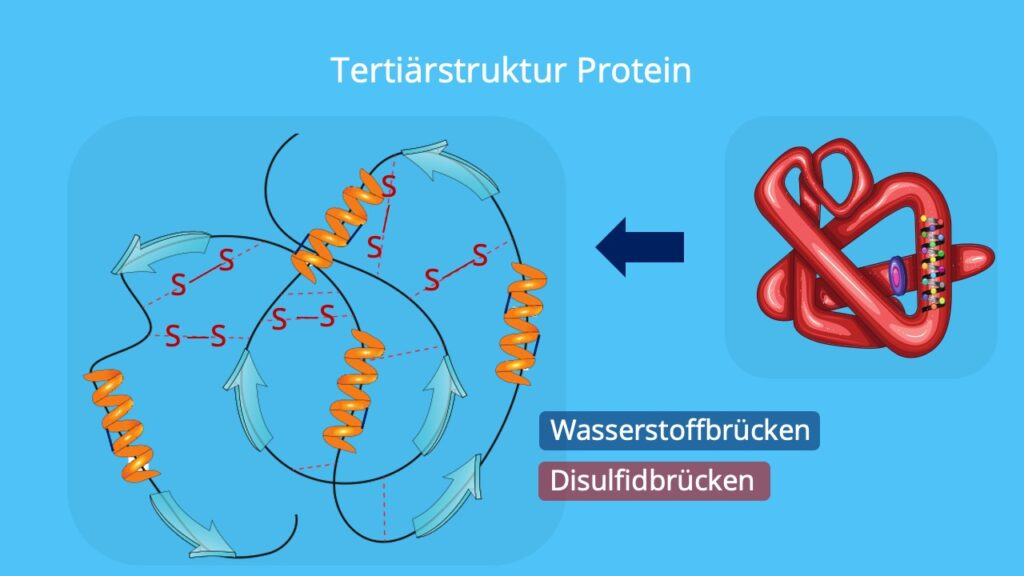
\includegraphics[scale=0.25]{Proteine_Tertiär}
    \end{itemize}
    \filbreak
    \subsection{Coenzyme}
    Zum Ablauf einer enzymatischen Reaktion wird in erster linie ein \textbf{Enzym} und das dazugehörige \textbf{Substrat} benötigt.
    Diese verbinden sich bei einer enzymatisch gesteuerten Reaktion zum \textbf{Enzym-Substrat-Komplex}.
    Jedoch werden bei vielen enymatischen Reaktionen auch \textbf{Coenzyme} benötigt.
    Dies sind Moleküle, die während der Reaktion für kurze Zeit an ein Enzym binden, allerdings während der Reaktion "verbraucht" werden, das heißt sie gehen nicht unverändert aus der Reaktion heraus.
    Daher werden sie auch häufig auch als \textbf{Cosubstrate} bezeichnet.\\
    Beispiele für Coenzyme sind: ATP und NADH+H\textsuperscript{+}
    \filbreak
    \subsection{Einflüsse auf die Enzymaktivität}
        \subsubsection{pH-Wert}
        Bei niedrigen pH-Wert läuft eine enzymatisch gesteuerte Reaktion verlangsamt ab.
        Bei höheren pH-Wert steigt die Enzymaktivität an, bis die Enzyme ihr \textbf{pH-Optimum} erreichen und bei zu hohem pH-Wert \textbf{denaturieren}.
        \filbreak
        \subsubsection{Temperatur}
        Bei niedrigen Temperaturen läuft eine enzymatisch gesteuerte Reaktion verlangsamt ab.
        Bei höheren Temperaturen folgt die Enzymaktivität annähernd der \textbf{RGT-Regel}, bis die Enzyme ihr \textbf{T-Optimum} erreichen, und schließlich bei ansteigender Temperatur \textbf{denaturieren}.
        \filbreak
        \subsubsection{Substratkonzentration}
        Bei steigender Substratkonzentration steigt auch die Enzymaktivität.
    \subsection{Hemmung von Enzmen}
        \subsubsection{allosterische Hemmung}
        Bei der \textbf{allosterischen Hemmung} lagert sich ein allosterischer Hemmstoff an das Enzym an.
        Dadurch wird das aktive Zentrum des Enzyms verändert und die Anzahl der reaktionsfähigen Enzyme herabgesetzt.
        Die maximale Reaktionsgeschwindigkeit, die eigentlich möglich gewesen wäre, kann also mit steigender Substratkonzentration nicht erreicht werden.
        Die allosterische Hemmung ist eine reversible Hemmung.
        \filbreak
        \subsubsection{kompetetive Hemmung}
        Bei der \textbf{kompetetiven Hemmung} lagert sich ein kompetetiver Hemmstoff an das aktive Zentrum des Enzym an.
        Dieser blokiert damit den Zugang des Substrates zum aktiven Zentrum des Enzyms.
        Da die Anzahl an reaktionsfähigen Enzmen nicht absinkt, kann bei Steigerung der Substratkonzentration die maximal mögliche Reaktionsgeschwindigkeit erreicht werden.
        Dies liegt daran das bei häufigerem Auftreten des Substrates ein Aufeinandertreffen zwischen Substrat und Enzym wahrscheinlicher wird als ein Aufeinandertreffen zwischen Hemmstoff und Enzym.
        Die kompetetive Hemmung ist eine reversible Hemmung.
        \filbreak
        \subsubsection{Schwermetall-Hemmung}
        Da bei der \textbf{Schwermetall-Hemmung} sich Schwermetalle so stark an Enzyme binden und deren Struktur verändern, dass die Verbindung nicht mehr einfach zu lösen ist, spricht man auch von irreversibler Hemmung.
        Man spricht in diesem Kontxt auch oft von \textbf{Enzymvergiftung}.
    \filbreak
\end{document}